
\documentclass{article}
\usepackage[a4paper,margin=1in]{geometry}
\usepackage{amsmath, amssymb, graphicx, hyperref, xcolor, booktabs, comment}

\title{Full Rank Hypothesis (FRH) Study}
\author{Camilla Polvara}
\date{}

\newcommand{\phdag}{{\vphantom{\dagger}}}

\usepackage{array}
\newcolumntype{C}[1]{>{\centering\arraybackslash}m{#1}}  % for centering in fixed width

\begin{document}

\maketitle

\section{Introduction}
The Full Rank Hypothesis (FRH) is a framework for analyzing the structure and dynamics of quantum many-body wavefunctions. In this study, we investigate the validity and implications of the FRH across several models, including the one-dimensional transverse field Ising model (TFIM), the PXP model, and the TFIM defined on an icosahedral geometry. Our primary focus is to explore the relationship between the FRH and the presence of quantum scar states, which are known to deviate from typical thermalization behavior and exhibit atypically low entanglement compared to other eigenstates at similar energies.\\
Notably, in some of these models, the reduced density matrix (RDM) of a subsystem of \( n \) spins - where \( n < N/2 \) and \( N \) is the full system size - fails to have full rank, indicating a breakdown of the FRH.


\section{1D Transverse Field Ising Model (TFIM)}
The transverse field Ising model is one of the simplest paradigms for quantum phase transitions. The Hamiltonian is given by:

\begin{equation} \label{e1}
    H = -J \sum_{i=1}^N \sigma^x_i \sigma^x_{i+1} - h \sum_{i=1}^N \sigma^z_i,
\end{equation}

where $J$ is the interaction strength, $h$ is the transverse field and $N$ is the number of sites. $\sigma^x, \sigma^z$ are the $(x,z)$ Pauli matrices:

\begin{equation}
\sigma_x = \begin{pmatrix} 0 & 1 \\ 1 & 0 \end{pmatrix}, \quad
\sigma_y = \begin{pmatrix} 0 & -i \\ i & 0 \end{pmatrix}, \quad
\sigma_z = \begin{pmatrix} 1 & 0 \\ 0 & -1 \end{pmatrix}
\end{equation}

The Pauli raising and lowering operators, which we will need shortly, are defined in terms of the Pauli matrices $\sigma^x$ and $\sigma^y$ as follows:

\begin{equation}
\sigma^{\pm} = \frac{1}{2} (\sigma_x \pm i\sigma_y), \quad
\sigma^+ = \begin{pmatrix} 0 & 1 \\ 0 & 0 \end{pmatrix}, \quad
\sigma^- = \begin{pmatrix} 0 & 0 \\ 1 & 0 \end{pmatrix}
\end{equation}

All the matrices are defined at site $i$, meaning that

\begin{align}
&\sigma_i = \mathbb{I}_2\otimes\hdots\otimes\underbrace{\sigma}_{i}\otimes\hdots\otimes\mathbb{I}_2\\
&\sigma_i\sigma_j = \mathbb{I}_2\otimes\hdots\otimes\underbrace{\sigma}_{i}\otimes\hdots\otimes\underbrace{\sigma}_{j}\otimes\hdots\otimes\mathbb{I}_2
\end{align}


The TFIM Hamiltonian exhibits the following symmetries:

\begin{itemize}
    \item \textbf{$\mathbb{Z}_2$ symmetry (Global Spin Flip):} The Hamiltonian is invariant under a global spin flip along the $x$-axis:
    \[
    \sigma_i^x \to -\sigma_i^x, \quad \sigma_i^z \to \sigma_i^z
    \]

    \item \textbf{Time-Reversal Symmetry:} Since the Hamiltonian contains only real terms, it is invariant under time-reversal symmetry $\mathcal{T}$, which acts as:
    \[
    \mathcal{T}: i \to -i, \quad \sigma_i^x, \sigma_i^z \to \sigma_i^x, \sigma_i^z
    \]

    \item \textbf{Translational Symmetry:} With periodic boundary conditions, the model is invariant under discrete lattice translations:
    \[
    i \to i+1
    \]

    \item \textbf{Reflection (Parity) Symmetry:} For chains with reflection-symmetric boundaries, the model is invariant under spatial inversion:
    \[
    i \to N - i + 1
    \]
\end{itemize}

The FRH in this system is investigated by analyzing the eigenstates and their rank structure ($3,4$- spins rdms) in different parameter regimes. In the case considered, $J=h=1$ (critical regime).\\
To diagonalize the transverse field Ising model (TFIM), we start from the Hamiltonian Eq. \eqref{e1} with periodic boundary conditions ($\sigma_{N+1} = \sigma_1$).\\
The first step is to map spins to fermions using the Jordan-Wigner transformation:
 
\begin{align} 
\sigma^-_i = F_i c_i \quad \sigma^+_i = F_i c^\dagger_i \quad \sigma^{z}_i = 2 c^\dagger_i c_i - 1
\end{align} 

where $c_j$​ are canonical fermionic annihilation operators satisfying
 
\begin{equation}
\{c_i , c_j^\dag \}=\{c^\dag_i ​, c_j​\}=\delta_{i,j}, \quad \{c^\dag_i , c_j^\dag \}=\{c_i ​, c_j​\}=0
\end{equation}

and we have defined the Jordan-Wigner string operator, 

\begin{equation}
F_i = (-1)^{n_i} = e^{i\pi\sum_{l=1}^{i-1} c^\dag _l c^\phdag_l}= \prod_{l=1}^{i-1} (1 - 2 c^\dagger_l c_l)
\end{equation}

which is crucial for ensuring the correct fermionic anticommutation relations when mapping spin operators to fermionic operators. $F_i$ introduces a non-local phase that keeps track of how many fermions are to the left of site $i$, enforcing the correct sign changes due to fermionic statistics.\\
The following properties hold

\begin{align}
&F_i c_i = c_i F_i, \quad F_i c^\dag_i = c^\dag_i F_i \\
&F_i F_{i+1} = (-1)^{c^\dag_i c^\phdag_i} = (-1)^{n_i}\\
&\left( c^\dag_i + c_i\right) (-1)^{n_i} = c^\dag_i - c_i
\end{align}

With the application of the Jordan-Wigner mapping, the two terms in Eq. \eqref{e1} become

\begin{align}
 \sigma^x_i \sigma^x_{i+1} &= F_i \left( c^\dag_i + c_i\right) F_{i+1} \left( c^\dag_{i+1} + c_{i+1}\right)\\
 &= \left( c^\dag_i + c_i\right) F_i F_{i+1} \left( c^\dag_{i+1} + c_{i+1}\right)\\
 &= \left( c^\dag_i + c_i\right) (-1)^{n_i} \left( c^\dag_{i+1} + c_{i+1}\right)\\
 &= \left( c^\dag_i - c_i\right) \left( c^\dag_{i+1} + c_{i+1}\right)
\end{align}

and

\begin{equation}
\sigma^z_i = 2 c^\dagger_i c_i - 1
\end{equation}

so that the TFIM Hamiltonian becomes quadratic in fermions:

\begin{equation}
H = -J \sum_{i=1}^N \left( c^\dag_i c_{i+1} +  c^\dag_{i+1} c_i +  c^\dag_i c^\dag_{i+1} + c_{i+1} c_i - 2h  c^\dag_i c_i + h \right)
\end{equation} 

We then Fourier transform: 

\begin{equation}
 c_j = \frac{1}{\sqrt{N}} \sum_k e^{i k a j} c_k, \qquad k = \frac{2\pi}{Na} \left(n + \frac{1}{2}\right), \quad n \in \mathbb{Z}
 \end{equation} 
 
 where $a$ is the spacing between lattice sites (we set $a=1$), to obtain the momentum-space Hamiltonian:
 
 \begin{equation} 
 H = -J \sum_k \left[ (\cos k - h)(c^\dagger_k c_k - c_{-k} c^\dagger_{-k}) + i \sin k (c^\dagger_k c^\dagger_{-k} + c_k c_{-k}) + h \right] 
\end{equation}

This Hamiltonian can be diagonalized by a Bogoliubov transformation: 

\begin{equation} 
\gamma_k = u_k c_k + v_k c^\dagger_{-k}, \quad \gamma^\dagger_k = u^*_k c^\dagger_k + v^*_k c_{-k} 
\end{equation} 

with coefficients $u_k,v_k\in\mathbb{C}$, such that $|u_k|^2 + |v_k|^2 = 1$ and such that the transformed Hamiltonian becomes: 

\begin{equation} 
H = \sum_k \varepsilon_k \left( \gamma^\dagger_k \gamma_k - \frac{1}{2} \right) 
\end{equation} where the quasiparticle dispersion relation is 

\begin{equation} 
\varepsilon_k = 2J \sqrt{(\cos k - h)^2 + \sin k^2} = 2J \sqrt{1 + h^2 - 2h \cos k}
\end{equation}

It's possible to show that the correct $u_k, v_k$ leading to this dispersion are:

\begin{equation}
u_k = \cos \frac{\theta_k}{2}, \quad v_k = \sin \frac{\theta_k}{2}, \quad \tan \theta_k = \frac{\sin k}{h - \cos k}
\end{equation}

The operators $\gamma_k$​ describe non-interacting fermionic quasiparticles:

\begin{equation}
\{ \gamma_k, \gamma^\dag_p\} = \{ \gamma^\dag_k, \gamma_p\} = \delta_{k,p}, \quad \{ \gamma^\dag_k, \gamma^\dag_p\} = \{ \gamma_k, \gamma_p\} = 0
\end{equation}

and the number operators 

\begin{equation} 
n_k = \gamma^\dagger_k \gamma_k 
\end{equation} 

are conserved quantities, since they commute with the Hamiltonian: 

\begin{equation} 
[H, n_k] = 0 \quad \forall k
\end{equation} 

This yields an infinite set of conserved charges, one for each allowed momentum $k$. These charges completely specify each eigenstate.
However, these occupation numbers $n_k$ are nonlocal in real space. Let us show this explicitly.

\begin{align} \label{e2}
n_k &= \gamma_k^\dag \gamma_k = \left( u^*_k c^\dagger_k + v^*_k c_{-k} \right) \left( u_k c_k + v_k c^\dagger_{-k} \right) \\
&= |u_k|^2 c_k^\dag c_k + u^*_k v_k c_k^\dag c^\dag_{-k} + u_k v^*_k c_{-k} c_k + |v_k|^2 c_{-k} c^\dag_{-k}
\end{align}

We can express each term in Eq. \eqref{e2} in real space. The inverse Fourier transform is:

\begin{equation}
 c_k = \frac{1}{\sqrt{N}} \sum_{j=1}^N e^{i k j} c_j
 \end{equation}
 
For example, the first term becomes

\begin{align} 
c_k^\dag c_k = \frac{1}{N} \sum_{j,j^{\prime}=1}^N e^{i k (j - j^{\prime})} c^\dag_j c_{j^{\prime}}
\end{align}

We now go back to Pauli matrices by applying the inverse Jordan-Wigner transformation

\begin{equation}
c_j = \frac{1}{2} \left( \prod_{l=1}^{j-1} \sigma_l^z \right) \sigma_j^-
\end{equation}

so that

\begin{align} \label{e3}
c_k^\dag c_k = \frac{1}{16N} \sum_{j,j^{\prime}=1}^N e^{i k (j - j^{\prime})} \left( \prod_{l=1}^{j-1} \sigma_l^z \right) \left( \sigma_j^x + i \sigma_j^y\right) \left( \prod_{l^\prime=1}^{j^\prime-1} \sigma_{l^\prime}^z \right) \left( \sigma_{j^\prime}^x - i \sigma_{j^\prime}^y\right) 
\end{align}

We split the calculation into 3 parts, $j=j^\prime$, and $j\neq j^\prime$ ($j<j^\prime$, $j>j^\prime$).
The commutation relations of the Pauli matrices will come in handy:

\begin{equation}
[\sigma_\alpha^i, \sigma_\beta^j] = 2i\epsilon_{ijk} \sigma_\alpha^k \, \delta_{\alpha,\beta}, \quad i,j,k = x,y,z 
\end{equation}

\begin{itemize}

\item $j=j^\prime$

\begin{align}
 &\left( \prod_{l=1}^{j-1} \sigma_l^z \right) \left( \sigma_j^x + i \sigma_j^y\right) \left( \prod_{l^\prime=1}^{j^\prime-1} \sigma_{l^\prime}^z \right) \left( \sigma_{j^\prime}^x - i \sigma_{j^\prime}^y\right) =\left( \prod_{l=1}^{j-1} \left(\sigma_l^z\right)^2 \right) \left( \sigma_j^x + i \sigma_j^y\right) \left( \sigma_{j}^x - i \sigma_{j}^y\right) \\
 &= \left( \sigma_j^x + i \sigma_j^y\right) \left( \sigma_{j}^x - i \sigma_{j}^y\right) = \left(\sigma_j^x\right)^2 + \left(\sigma_j^y\right)^2 - i [\sigma_j^x,\sigma_j^y] = 2 \left( \mathbb{I}_2 + \sigma^z_j\right)
\end{align}

\item $j < j^\prime$

\begin{equation}
\prod_{l'=1}^{j'-1} \sigma_{l'}^z = \left( \prod_{l'=1}^{j-1} \sigma_{l'}^z \right) \left( \prod_{l''=j}^{j'-1} \sigma_{l''}^z \right)
\end{equation}

So that

\begin{align}
&\left( \prod_{l=1}^{j-1} \sigma_l^z \right) \left( \sigma_j^x + i \sigma_j^y\right) \left( \prod_{l^\prime=1}^{j^\prime-1} \sigma_{l^\prime}^z \right) \left( \sigma_{j^\prime}^x - i \sigma_{j^\prime}^y\right) \\
&= \left( \prod_{l=1}^{j-1} \sigma_l^z \right)^2 \left( \sigma_j^x + i \sigma_j^y\right) \left( \prod_{l^\prime=j}^{j^\prime-1} \sigma_{l^\prime}^z \right) \left( \sigma_{j^\prime}^x - i \sigma_{j^\prime}^y\right)\\
& = \left( \sigma_j^x + i \sigma_j^y\right) \left( \prod_{l^\prime=j}^{j^\prime-1} \sigma_{l^\prime}^z \right) \left( \sigma_{j^\prime}^x - i \sigma_{j^\prime}^y\right)\\ 
&= \left( \sigma_j^x + i \sigma_j^y\right) \sigma_j^z \left( \prod_{l^\prime=j+1}^{j^\prime-1} \sigma_{l^\prime}^z \right) \left( \sigma_{j^\prime}^x - i \sigma_{j^\prime}^y\right)\\
& = \left[ \left(\sigma_j^z - 2 \mathbb{I}_2\right) \left( \sigma_j^x + i \sigma_j^y\right) \right]  \left( \prod_{l^\prime=j+1}^{j^\prime-1} \sigma_{l^\prime}^z \right) \left( \sigma_{j^\prime}^x - i \sigma_{j^\prime}^y\right)\\
&= \left(\sigma_j^z - 2 \mathbb{I}_2\right) \left( \prod_{l=j+1}^{j^\prime-1} \sigma_{l}^z \right) \left( \sigma_j^x + i \sigma_j^y\right) \left( \sigma_{j^\prime}^x - i \sigma_{j^\prime}^y\right) 
\end{align}

\item $j > j^\prime$

\begin{equation}
\prod_{l=1}^{j-1} \sigma_l^z =
\left( \prod_{l=1}^{j'-1} \sigma_l^z \right)
\left( \prod_{l'=j'}^{j-1} \sigma_{l'}^z \right)
\end{equation}

Then, proceeding as before

\begin{align}
 &\left( \prod_{l=1}^{j-1} \sigma_l^z \right) \left( \sigma_j^x + i \sigma_j^y\right) \left( \prod_{l^\prime=1}^{j^\prime-1} \sigma_{l^\prime}^z \right) \left( \sigma_{j^\prime}^x - i \sigma_{j^\prime}^y\right) \\ 
 &= \left( \prod_{l=1}^{j'-1} \sigma_l^z \right)^2 \left( \prod_{l'=j'}^{j-1} \sigma_{l'}^z \right) \left( \sigma_j^x + i \sigma_j^y \right) \left( \sigma_{j^\prime}^x - i \sigma_{j^\prime}^y \right) \\
 &= \left( \prod_{l'=j'}^{j-1} \sigma_{l'}^z \right) \left( \sigma_j^x + i \sigma_j^y \right) \left( \sigma_{j^\prime}^x - i \sigma_{j^\prime}^y \right)
 \end{align} 

\end{itemize}

Putting everything together

\begin{equation}
c_k^\dagger c_k = \frac{1}{16N} \sum_{j,j'=1}^N e^{ik(j - j')} \, \Gamma_{jj'}
\end{equation}

where the operator-valued kernel \( \Gamma_{jj'} \) depends on the relative positions of \( j \) and \( j' \) as follows:

\begin{equation}
\Gamma_{jj'} =
\begin{cases}
2(\mathbb{I}_2 + \sigma_j^z), & \text{if } j = j' \\[1.2em]
(\sigma_j^z - 2 \mathbb{I}_2)
\left( \prod\limits_{l = j+1}^{j'-1} \sigma_l^z \right)
(\sigma_j^x + i \sigma_j^y)(\sigma_{j'}^x - i \sigma_{j'}^y),
& \text{if } j < j' \\[1.2em]
\left( \prod\limits_{l = j'}^{j-1} \sigma_l^z \right)
(\sigma_j^x + i \sigma_j^y)(\sigma_{j'}^x - i \sigma_{j'}^y),
& \text{if } j > j'
\end{cases}
\end{equation}

Analogous expressions hold for the other terms of Eq. \eqref{e3}. The most important point is that the sum for all of them runs over the whole lattice (ie. up to $N$), and is therefore not local. In other words, there do not exist locally commuting charges in the TFIM; the occupation numbers $n_k$ commute with the TFIM Hamiltonian but they are defined globally. This is confirmed by numerical analysis too. In the critical regime, the 3/4 spins rdms of the $12$ spins TFIM are full rank:


\begin{figure}[h!]
  \centering
  \begin{minipage}[b]{0.45\textwidth}
    \centering
    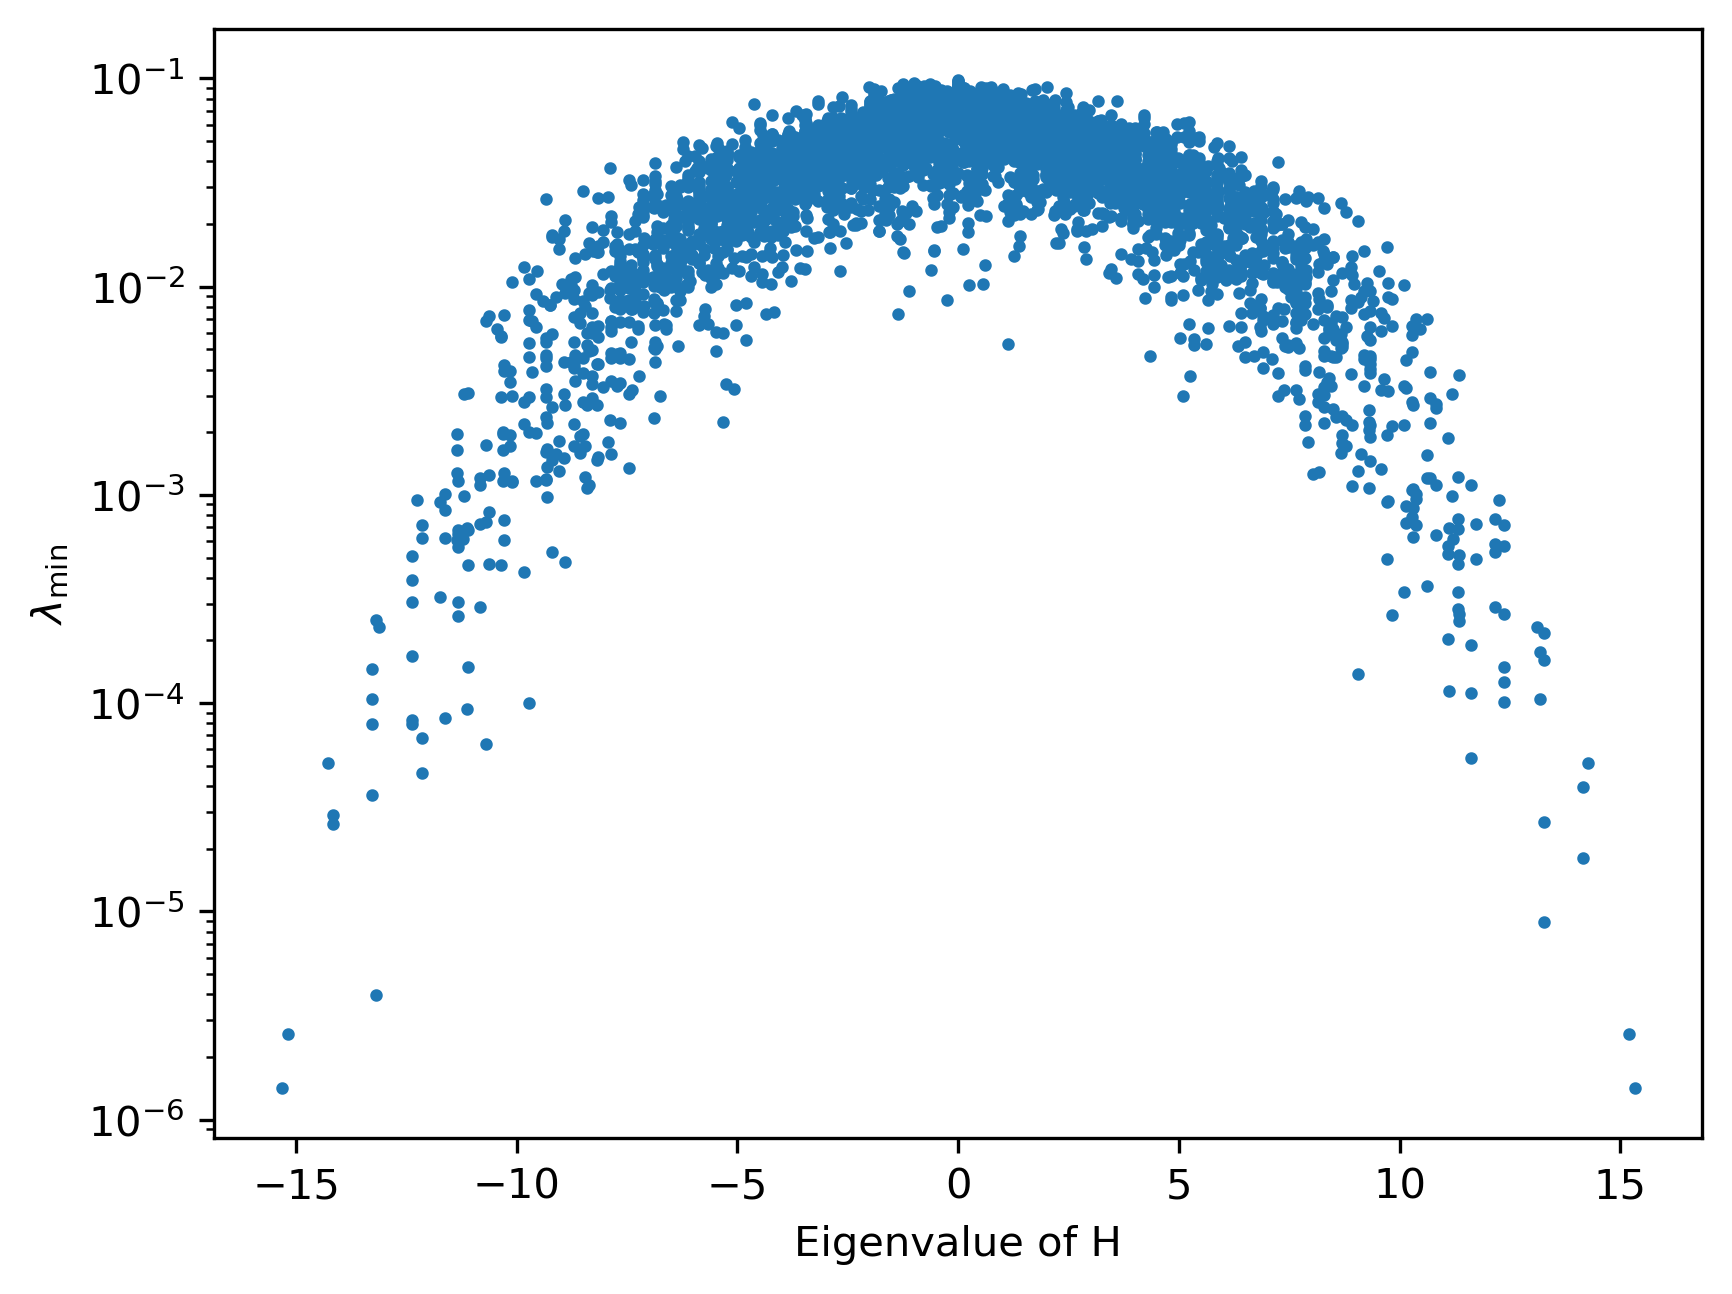
\includegraphics[width=\textwidth]{TFIM_pbc_3spins.png}
    \caption{Minimum eigenvalue for $3$-spins rdm}
  \end{minipage}
  \hfill
  \begin{minipage}[b]{0.45\textwidth}
    \centering
    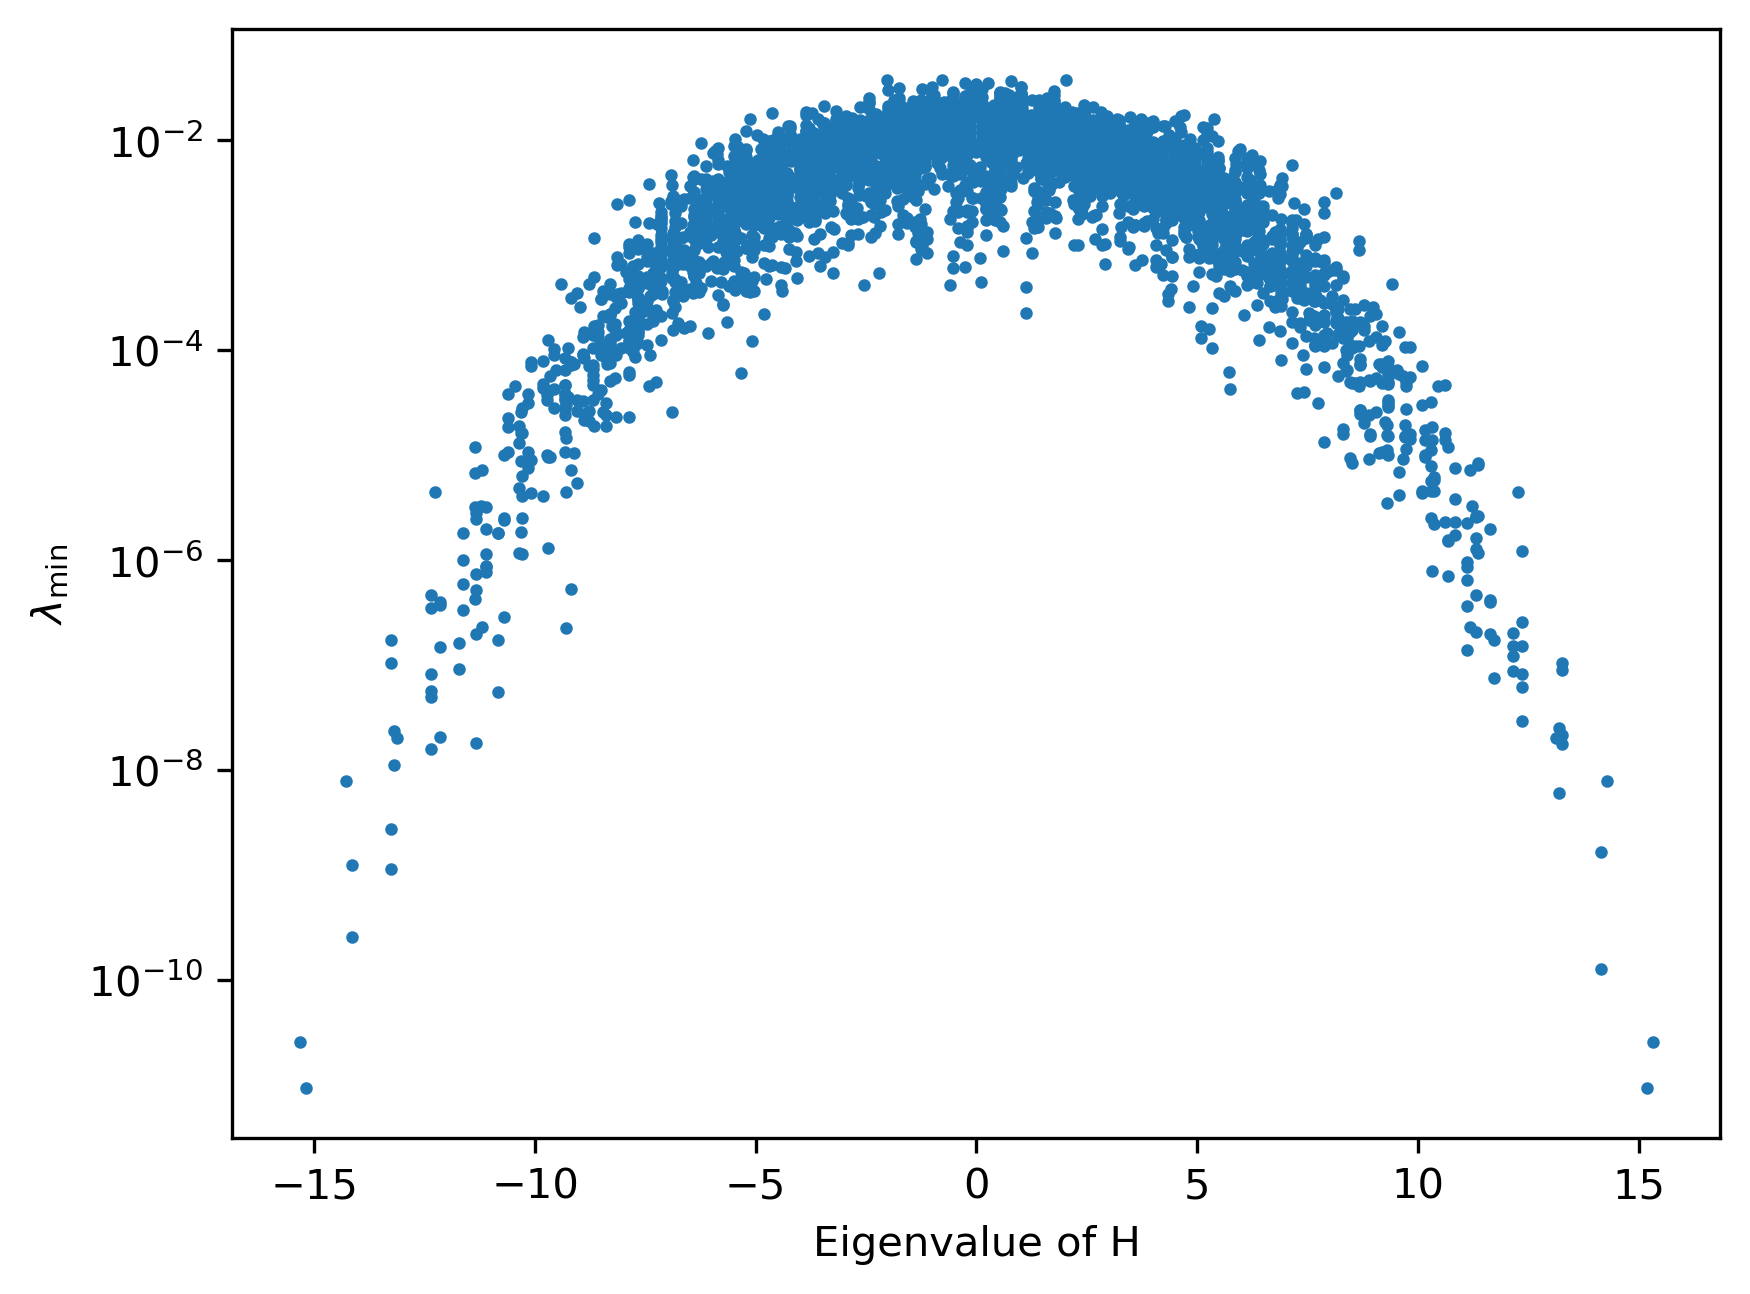
\includegraphics[width=\textwidth]{TFIM_pbc_4spins.png}
    \caption{Minimum eigenvalue of $4$-spins rdm}
  \end{minipage}
  %\caption{}
  \label{fig:minipage-images}
\end{figure}


In other words, the FRH is generically satisfied.\\
\textcolor{red}{mention majorana fermions notation. TFIM with obc has scars!}

\section{PXP Model}
The PXP model describes constrained dynamics relevant to Rydberg atom arrays. We will consider the simpler case of an array of spins, i.e. of $0,1$. The Hamiltonian takes the form (the tensor product between the operators at different sites, including $\mathbb{I}_2$ is left implicit):

\begin{equation}\label{eb}
H = \sum_{i=1}^N P_{i-1} \sigma^x_i P_{i+1}, 
\end{equation}

where, using the convention $|0\rangle = \begin{pmatrix} 1\\0 \end{pmatrix} , |1\rangle = \begin{pmatrix} 0\\1 \end{pmatrix}$

\begin{equation}
\sigma^x = |0\rangle \langle1| + |1\rangle \langle0| = \begin{pmatrix} 0&1\\1&0 \end{pmatrix}
\end{equation} 

\begin{equation} \label{ea}
P = \frac{1}{2} (\mathbb{I}_2 + \sigma^z) = |0\rangle\langle 0| = \begin{pmatrix} 1&0\\0&0 \end{pmatrix}
\end{equation}

The projector $P_i$ ensures that adjacent excitations $|\hdots 1 1 \hdots \rangle$ are forbidden. By definition, the PXP model is defined only for the states without adjacent excitations, and the presence of the projectors $P$ just make sure the Hamiltonian remains in this subspace. We call the subspace of states allowed by the PXP model \emph{PXP subspace}, whereas the kinetic constraint on the Hilbert space is known as \emph{Rydberg blockade}.\\
Eq. \eqref{eb} admits open or periodic boundary conditions (obc, pbc). For the former, we set $P_0 = P_{N+1} = \mathbb{I}_2$, and for the latter $P_0 = P_N, P_{N+1} = P_1$.\\

For example, for \( N = 3 \), the PXP Hamiltonian with open and periodic boundary conditions is given by:

\begin{align} \label{ec}
H_{\mathrm{obc}} &= \sigma^x_1 P_2 + P_1\sigma^x_2 P_3 + P_2 \sigma^x_3, \\
H_{\mathrm{pbc}} &= \sigma^x_1 P_2 P_3 + P_1 \sigma^x_2 P_3 + P_1 P_2 \sigma^x_3.
\end{align}

The PXP subspace for obc is spanned by states $|0,0,0\rangle, |1,0,0\rangle, |0,1,0\rangle, |0,0,1\rangle, |1,0,1\rangle$, whereas for pbc it is spanned by  $|0,0,0\rangle, |1,0,0\rangle, |0,1,0\rangle, |0,0,1\rangle$. The three-spin states that contain adjacent excitations—i.e., those that violate the Rydberg blockade constraint—are, for open boundary conditions: \( |1,1,0\rangle \), \( |0,1,1\rangle \), and \( |1,1,1\rangle \). For periodic boundary conditions, the state \( |1,0,1\rangle \) is also forbidden due to the wrap-around interaction between site 3 and site 1.

These states lie outside the PXP subspace. Nevertheless, one can formally act on them with the PXP Hamiltonian, and the result is zero: they are annihilated by the Hamiltonian.\\

It's easy to compute the dimension of the PXP subspace for a generic number of sites $N$, and to show that it's related to the Fibonacci sequence:

\begin{equation}
d_N^{\mathrm{\,obc}} = F_{N+2}, \quad d_N^{\mathrm{\,pbc}} = F_{N-1} + F_{N+1}
\end{equation}

where $F_N$ is the $N$-th Fibonacci number ($F_0 = 0, F_1 = 1, F_N = F_{N-1} + F_{N-2} \; \mathrm{for} \; N\geq 2$).\\
Going back to the $N=3$ example, we have 

\begin{align}
&d_3^{\mathrm{\,obc}} = F_{5} = 5, \\
&d_3^{\mathrm{\,pbc}} = F_{2} + F_{4} = 1+3 = 4,
\end{align}

as expected.\\

We have seen that the forbidden states are annihilated by the PXP Hamiltonian. In other words, applying the PXP Hamiltonian to either the PXP subspace or its complement does not allow transitions between them. This implies that the two sectors are dynamically disconnected. As a result, the Hilbert space undergoes fragmentation.

In the absence of the Rydberg blockade constraint, the model would be integrable in the sense that the dynamics could explore the full Hilbert space, and all states would thermalize. However, due to the kinetic constraint imposed by the blockade, certain states become dynamically isolated and cannot thermalize. This fragmentation of the Hilbert space leads to the emergence of nonthermal states, which are known as \emph{quantum scars}.

Among the nonthermal states in the PXP model, a particularly striking example is the so-called $Z_2$ Néel state, defined as \( |\mathbb{Z}_2\rangle = |1,0,1,0,\dots\rangle \), along with its translated counterpart \( |\mathbb{Z}_2'\rangle = |0,1,0,1,\dots\rangle \). These two states lie deep within the PXP subspace and exhibit atypical dynamics under the action of the Hamiltonian, characterized by long-lived oscillations and slow thermalization. This behavior has been associated with the presence of quantum many-body scars.

One way to understand the emergence of scars in the PXP model is through the construction of a \emph{tower of states} built on top of the $|\mathbb{Z}_2\rangle$ and $|\mathbb{Z}_2'\rangle$ states. These towers consist of a set of special eigenstates that are approximately equally spaced in energy and have large overlap with initial product states such as $|\mathbb{Z}_2\rangle$. A useful analytical framework for constructing such towers is the \emph{Forward Scattering Approximation} (FSA).

In the FSA, one begins with a reference state—typically $|\mathbb{Z}_2\rangle$—and iteratively applies the Hamiltonian, but only retains the part of the resulting state that is orthogonal to all previously generated states. This generates an approximately closed subspace, the FSA subspace, which captures the essence of the scarred eigenstates and reproduces many of their qualitative features, including their energy spacing and overlap structure.

Interestingly, there exists a related model in which the forward scattering approximation becomes \emph{exact}: the so-called \emph{free paramagnetic model}, defined by relaxing the Rydberg blockade constraint in a controlled way. This model can be viewed as a deformation of the PXP Hamiltonian in which the scar structure is lifted into an exact set of eigenstates. As such, it serves as a useful toy model for understanding the mechanisms that protect and stabilize scars in the constrained PXP dynamics.\\

The paramagnetic model is defined by the Hamiltonian

\begin{equation}
    H_{\mathrm{PM}} = \sum_{i=1}^N \sigma^x_i = H_+ + H_-   
\end{equation}

where $H_+, H_-$ are called forward and backward propagator, and they are defined as

\begin{align}
&H_+ = \sum_{j\,\in\,\mathrm{odd}} \sigma_j^- + \sum_{j\,\in\,\mathrm{even}} \sigma_j^+\\
&H_- = \sum_{j\,\in\,\mathrm{odd}} \sigma_j^+ + \sum_{j\,\in\,\mathrm{even}} \sigma_j^-
\end{align}

The Hamiltonian $H_{\mathrm{PM}}$ acts globally on all spins without any constraints. The key insight is that, when restricted to the subspace generated by the repeated action of \( H_+ \) on the Néel state \( |\mathbb{Z}_2\rangle = |1,0,1,0,\dots\rangle \), the dynamics becomes exactly solvable and exhibits a hidden \(\mathrm{SU}(2)\) algebraic structure.

Define an effective SU(2) ladder as follows:

\begin{equation}\label{enoa}
    N_{k+1}|k+1\rangle = H_+ |k\rangle, \quad \text{for } k = 0, 1, \dots, N,
\end{equation}

where \( N_{k+1} \) is the normalization constant for the state $|k+1\rangle$, and for a generic $k$ it's iteratively defined as

\begin{equation}\label{econst}
N_k = \sqrt{k \left( N - k + 1 \right)}
\end{equation}

The tower starts with the state $|0\rangle = |\mathbb{Z}_2\rangle $ and ends with the translated Néel state \( |\mathbb{Z'}_2\rangle \):

\begin{equation}
|\mathbb{Z}_2'\rangle = |N\rangle = \frac{(H_+)^N}{\sqrt{N}} |\mathbb{Z}_2\rangle
\end{equation}

The states \( \{ |k\rangle \} \) span a finite-dimensional Krylov subspace generated by repeated applications of the forward scattering operator \( H_+ \) on the Néel state \( |\mathbb{Z}_2\rangle \). In the paramagnetic model, this Krylov subspace is invariant under the action of the Hamiltonian \( H_{\mathrm{PM}} = H_+ + H_- \), and forms an exact irreducible representation of SU(2).\\
Within this subspace, the states \( |k\rangle \) form an exact tower of eigenstates of the Casimir operator of the SU(2) structure, defined as

\begin{equation}
H^2 = \frac{1}{2} \{ H_+, H_-\} + \frac{1}{4} \left( H_z\right)^2
\end{equation}

where

\begin{equation}
H_z = \sum_j \left( \sigma_{2j}^z - \sigma_{2j+1}^z\right)
\end{equation}

The forward and backward propagators generate transitions within the tower of states:

\begin{equation}
    H_+ |k\rangle \propto |k+1\rangle, \quad H_- |k\rangle \propto |k-1\rangle
\end{equation}

and the commutation relations of the $SU(2)$ algebra hold

\begin{equation}
[H_+,H_-] = H_z
\end{equation}

Also note that the Casimir operator $H^2$ commutes with the paramagnet Hamiltonian:

\begin{equation}
[H_{\mathrm{PM}},H^2] = 0,
\end{equation}

reflecting the fact that $H_{\mathrm{PM}}$​ preserves the $SU(2)$ representation structure.
This algebraic structure leads to equally spaced energy levels and it provides a useful toy model for understanding quantum scars in the PXP model.\\

In the PXP model, the kinetic constraint from the Rydberg blockade breaks the exact SU(2) structure. However, one can still construct an approximate tower of states using the \emph{Forward Scattering Approximation} (FSA).\\
The forward and backward propagators are now defined as 

\begin{align}
&H_+ = \sum_{j\,\in\,\mathrm{odd}} P_{j-1} \sigma_j^- P_{j+1} + \sum_{j\,\in\,\mathrm{even}} P_{j-1} \sigma_j^+ P_{j+1}\\
&H_- = \sum_{j\,\in\,\mathrm{odd}} P_{j-1} \sigma_j^+ P_{j+1} + \sum_{j\,\in\,\mathrm{even}} P_{j-1} \sigma_j^- P_{j+1}
\end{align}

To construct the FSA tower in the PXP model, one starts again from the Néel state \( |\mathbb{Z}_2\rangle \), and recursively generates a set of orthogonal states \( \{ |k\rangle \} \) as follows:

\begin{align}
|0\rangle &= |\mathbb{Z}_2\rangle, \\
|1\rangle &= H_+ |0\rangle, \\
N_{k+1}|k+1\rangle &= \left(H - a_k\right) |k\rangle - N_k |k-1\rangle, \label{eno}
\end{align}

where the coefficient \( a_k = \langle H \, k | k \rangle \) is chosen to enforce orthogonality between states $|k+1\rangle$ and $|k\rangle$ (not necessary in the paramagnet, where the SU(2) structure is exact and the basis vectors remain orthogonal by construction). 
Eq. \eqref{eno} is the PXP-modified version of Eq. \eqref{enoa}, since for the PXP model, $H_+ |k\rangle \not\propto |k+1\rangle$. Both forward and backward propagators $H_{\pm}$ are needed to generate the FSA states  in the PXP model (not just $H_+$).\\
Unlike in the paramagnetic model, the action of \( H_+ \) on \( |k\rangle \) does not remain entirely within the Krylov subspace \( \mathrm{span}\{ |0\rangle, \dots, |N\rangle \} \). This reflects the fact that the SU(2) ladder structure is only approximate, and that \( H_+ \), \( H_- \), and \( H_z = [H_+, H_-] \) no longer satisfy the exact SU(2) commutation relations.

The non-closure of the FSA basis can be quantified by evaluating the norm of the residual vector
\begin{equation}
|\delta_k\rangle = H_- |k-1\rangle - N_{k-1} |k-2\rangle,
\end{equation}
which is exactly zero in the paramagnetic model but nonzero in the PXP model. This deviation leads to slight distortions in the energy spectrum of the approximate tower, as well as to reduced orthogonality between the FSA states.

Nevertheless, the FSA remains remarkably effective in capturing the essential features of the scarred eigenstates of the PXP model. These special eigenstates have large overlap with the FSA basis, exhibit near-equal energy spacing, and support long-lived coherent oscillations when the system is initialized in \( |\mathbb{Z}_2\rangle \).\\

We numerically analyzed the PXP model for a chain of 12 spins with periodic boundary conditions (PBC), aiming to characterize quantum scarred eigenstates through three main diagnostics: their overlap with the Néel \( \mathbb{Z}_2 \) state, their bipartite entanglement entropy, and, most importantly, the properties of their reduced density matrices (RDMs) for three adjacent spins.

\begin{figure}[h!]
  \centering
  \begin{minipage}[c]{0.45\textwidth}
    \centering
    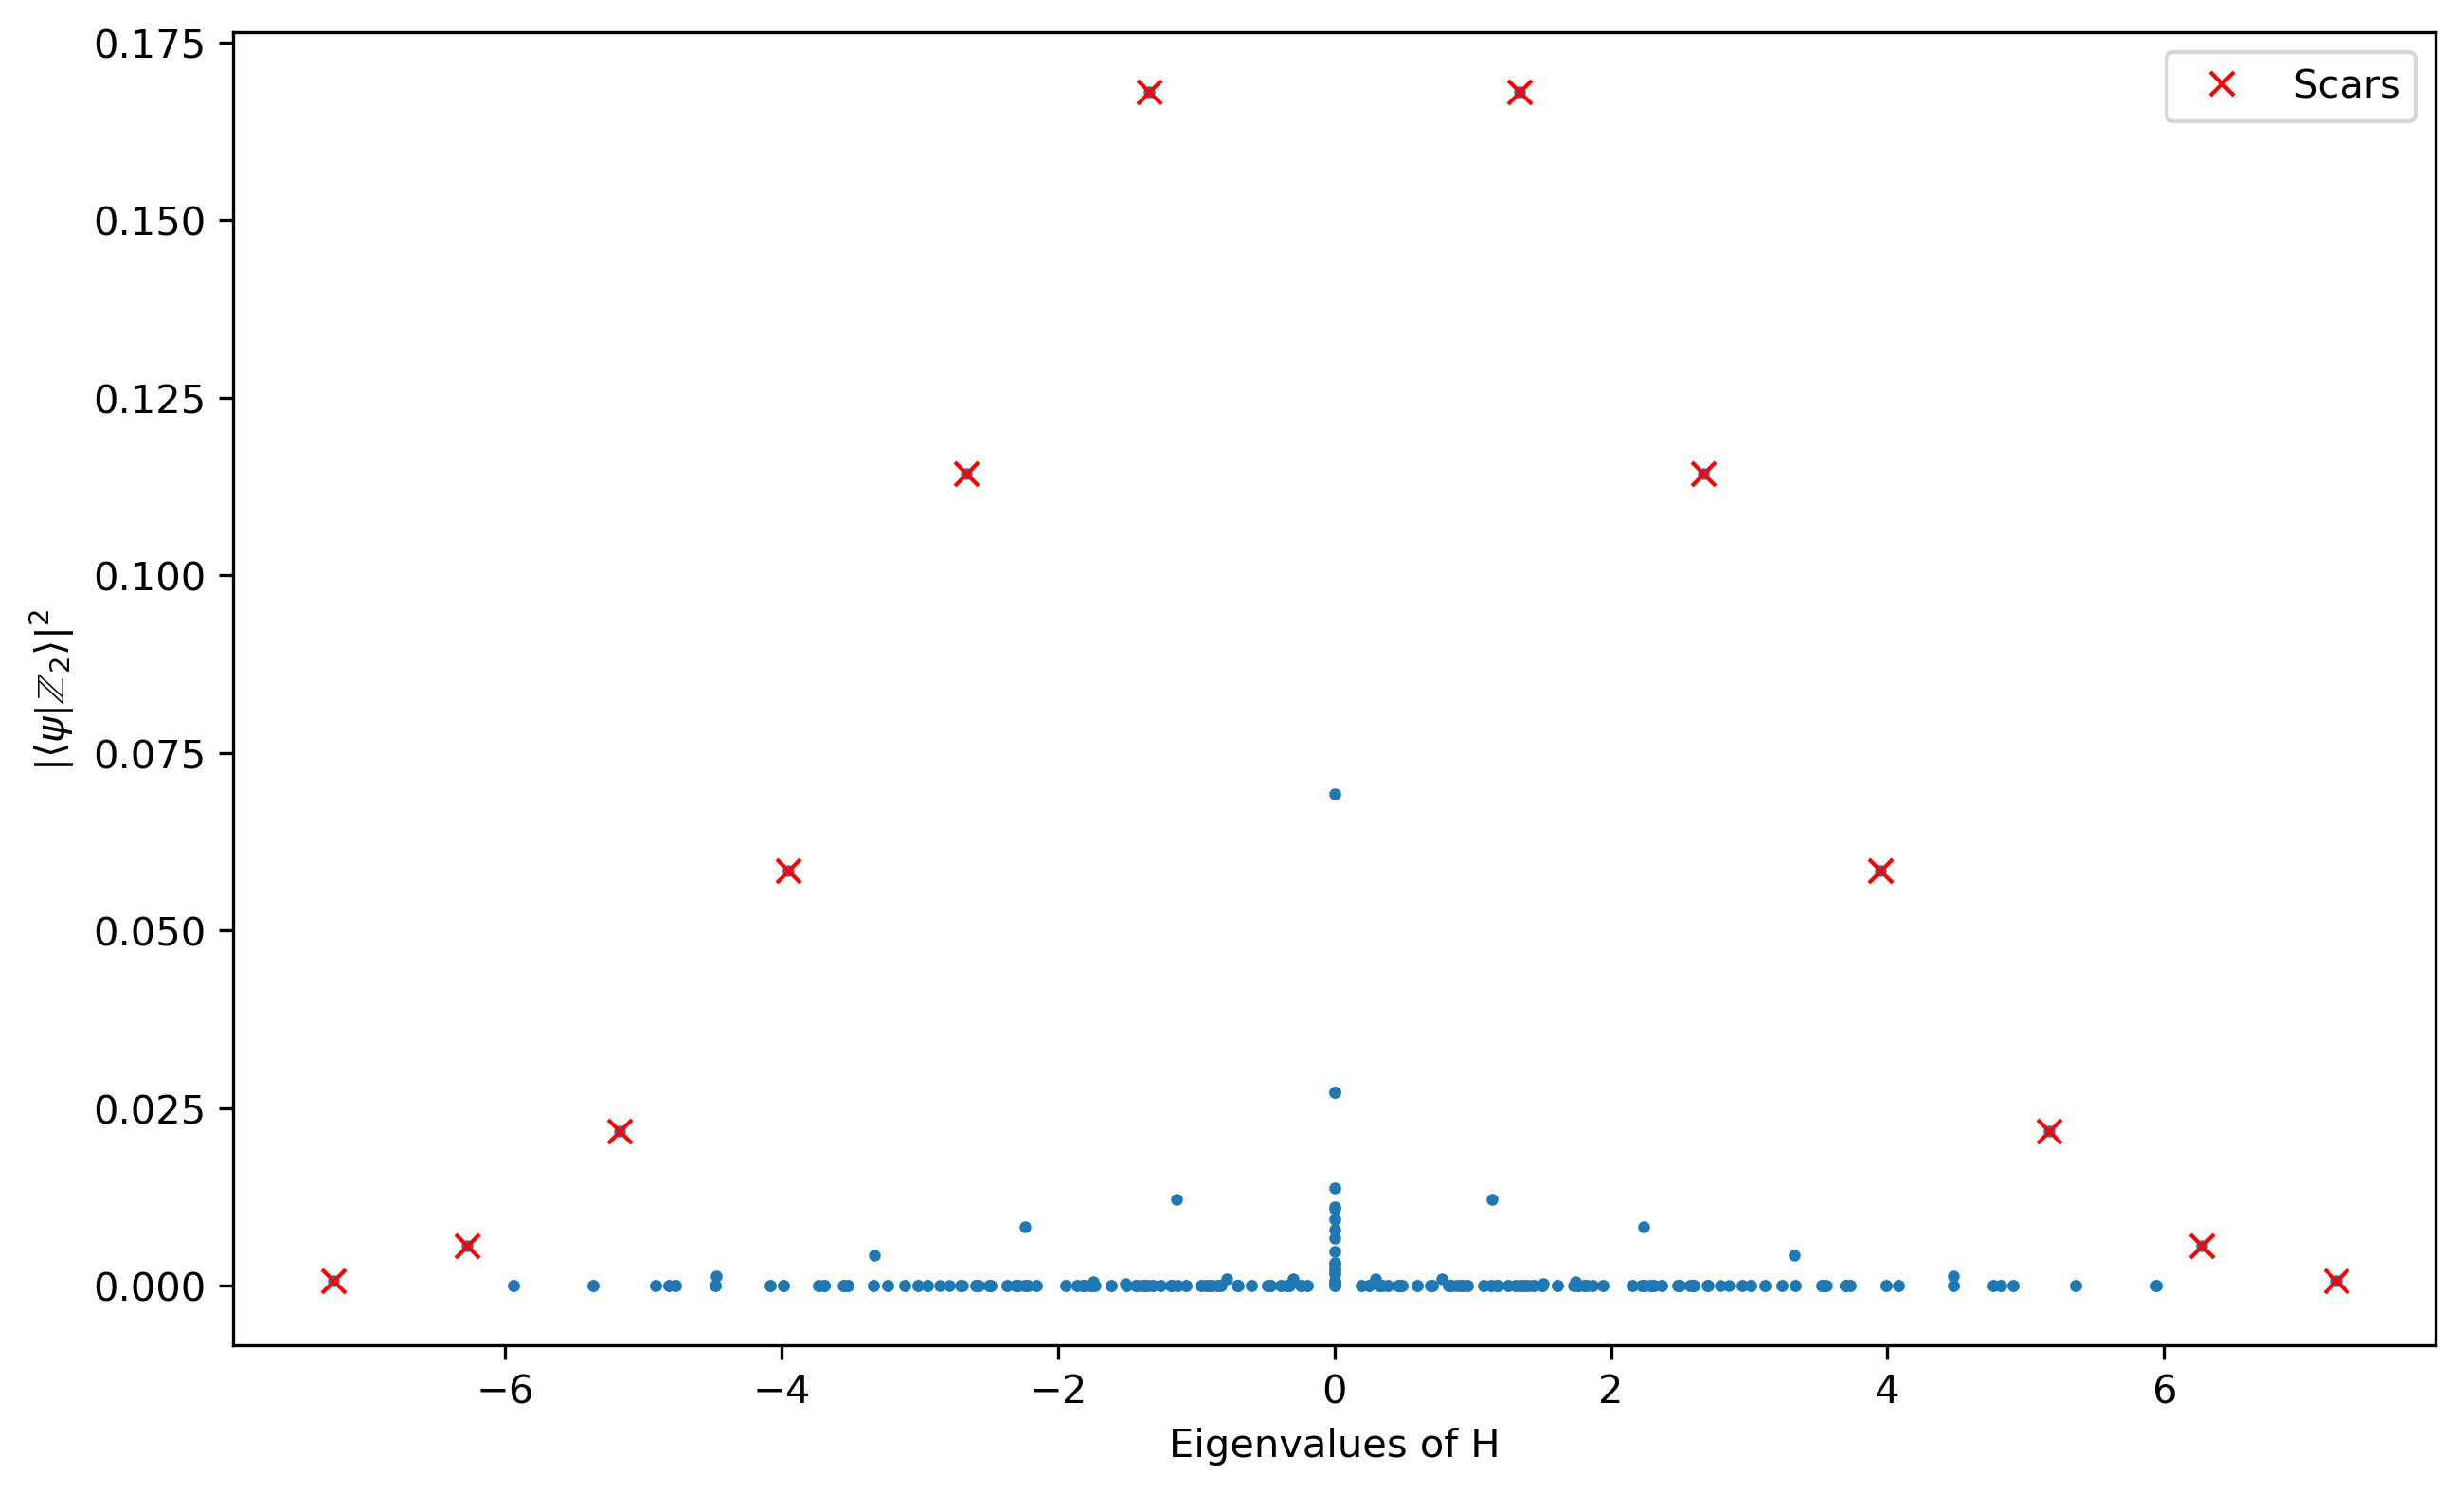
\includegraphics[height=5cm]{pxp_neel.png}
    \caption{Overlap between eigenstates and the Néel \( \mathbb{Z}_2 \) state. Quantum scars exhibit stronger overlap, in contrast to thermal states.}
  \end{minipage}
  \hfill
  \begin{minipage}[c]{0.45\textwidth}
    \centering
    %\vspace{4.5mm}
    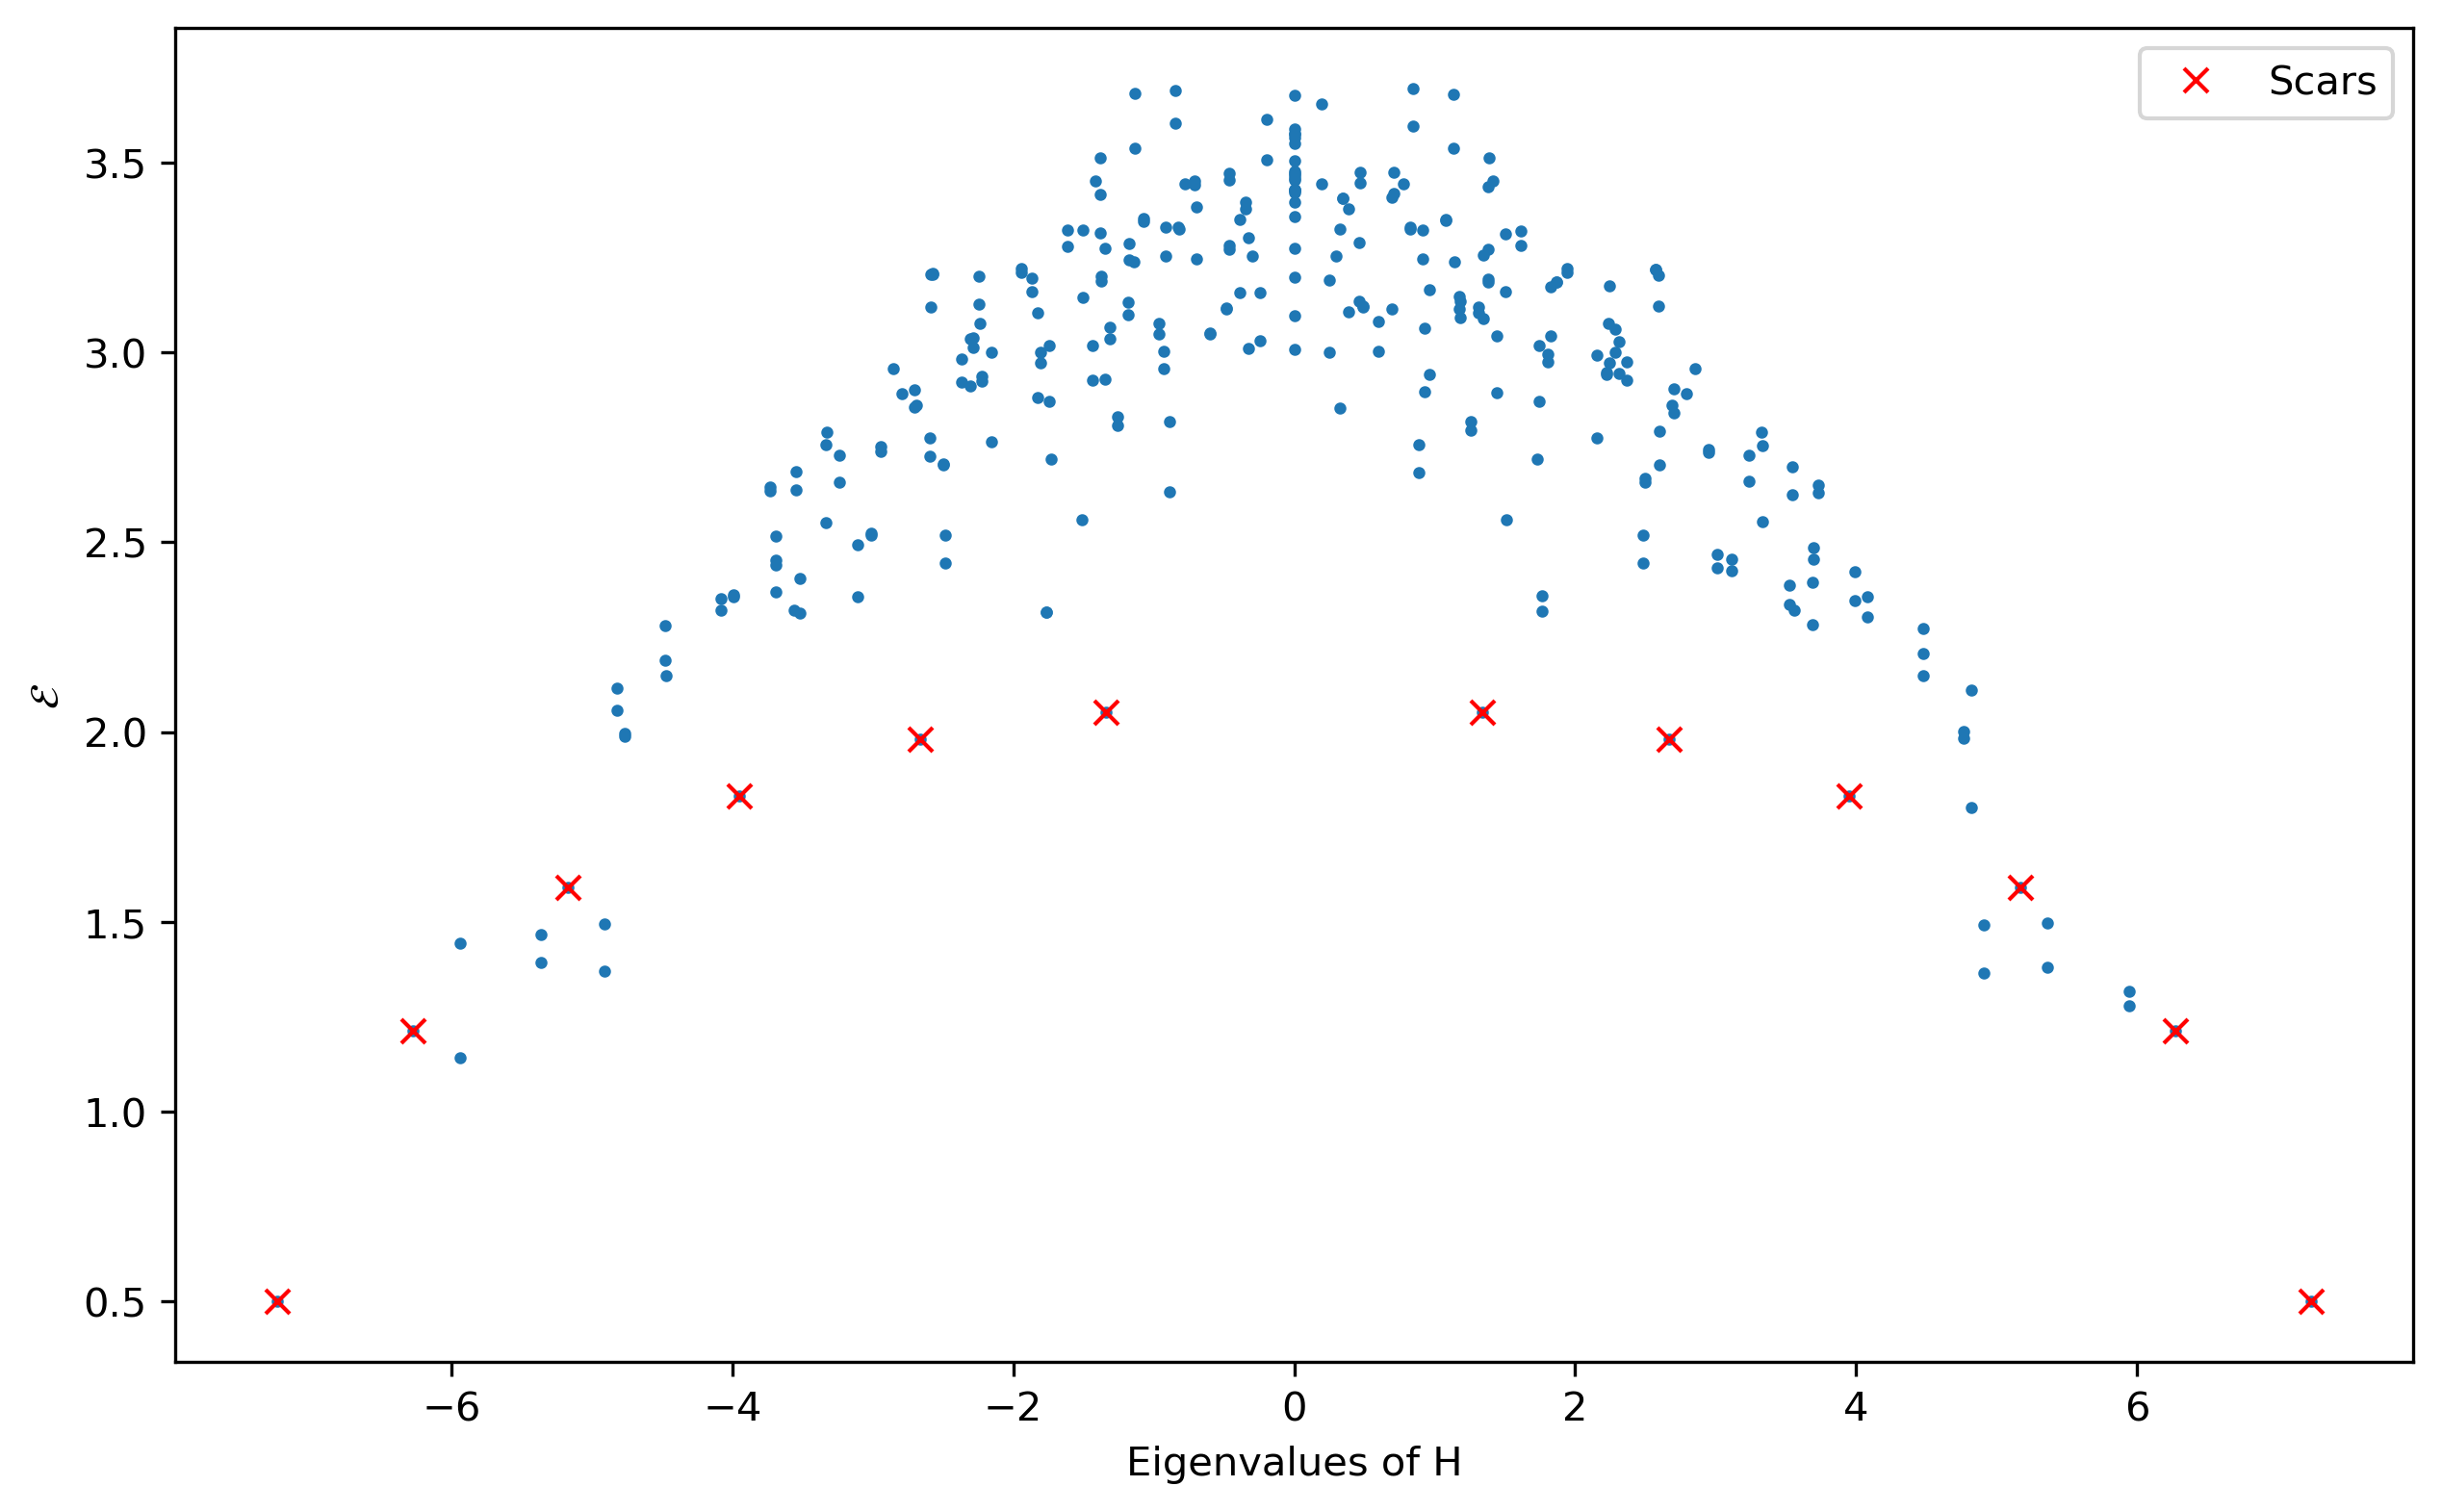
\includegraphics[height=5cm]{pxp_entanglement.png}
    \caption{Bipartite entanglement entropy of eigenstates. Scars exhibit low entanglement relative to thermal states.}
  \end{minipage}
  \label{fig:minipage-images}
\end{figure}

To probe the local structure of scarred eigenstates, we examined the RDM of the spins \([5,6,7]\) (equivalent results were observed for all triplets of adjacent spins, as expected from translation invariance). For each eigenstate, we computed the rank of the 3-spin RDM. The results are reported in the table below.

We found that all 3-spin RDMs associated with scarred eigenstates have \textbf{rank 5} (not full rank, 8), and consistently contain \textbf{three zero rows and columns}, corresponding to the \textbf{forbidden states} \( |011\rangle, |110\rangle, |111\rangle \). These are precisely the configurations excluded by the Rydberg blockade constraint.
This pattern highlights the failure of FRH in the PXP model not because of emergent symmetries or conserved quantities (such as the hidden SU(2) symmetry, present in the free paramagnetic model but not in the PXP model), but because of the constraints encoded directly at the level of local Hilbert space structure. The Rydberg blockade enforces a projection onto a kinetically constrained subspace, carving out a rigid structure that persists even in reduced local descriptions of the system.

\begin{comment}
\begin{table}[h!]
\centering
\renewcommand{\arraystretch}{1.2}
\begin{tabular}{r C{1.5cm} C{7.5cm}}
\toprule
Eigenvalue & RDM Rank & Zero Columns \\
\midrule
-7.242941 & 5 & $|011\rangle \langle 011|,\ |110\rangle \langle 110|,\ |111\rangle \langle 111|$ \\
-6.274371 & 5 & $|011\rangle \langle 011|,\ |110\rangle \langle 110|,\ |111\rangle \langle 111|$ \\
-5.170150 & 5 & $|011\rangle \langle 011|,\ |110\rangle \langle 110|,\ |111\rangle \langle 111|$ \\
-3.951588 & 5 & $|011\rangle \langle 011|,\ |110\rangle \langle 110|,\ |111\rangle \langle 111|$ \\
-2.665779 & 5 & $|011\rangle \langle 011|,\ |110\rangle \langle 110|,\ |111\rangle \langle 111|$ \\
-1.341881 & 5 & $|011\rangle \langle 011|,\ |110\rangle \langle 110|,\ |111\rangle \langle 111|$ \\
1.341881  & 5 & $|011\rangle \langle 011|,\ |110\rangle \langle 110|,\ |111\rangle \langle 111|$ \\
2.665779  & 5 & $|011\rangle \langle 011|,\ |110\rangle \langle 110|,\ |111\rangle \langle 111|$ \\
3.951588  & 5 & $|011\rangle \langle 011|,\ |110\rangle \langle 110|,\ |111\rangle \langle 111|$ \\
5.170150  & 5 & $|011\rangle \langle 011|,\ |110\rangle \langle 110|,\ |111\rangle \langle 111|$ \\
6.274371  & 5 & $|011\rangle \langle 011|,\ |110\rangle \langle 110|,\ |111\rangle \langle 111|$ \\
7.242941  & 5 & $|011\rangle \langle 011|,\ |110\rangle \langle 110|,\ |111\rangle \langle 111|$ \\
\bottomrule
\end{tabular}
\caption{All eigenstates of the PXP Hamiltonian exhibit rank-5 reduced density matrices due to the Rydberg blockade. The listed zero columns correspond to the forbidden configurations excluded from the dynamics.}
\label{tab:scar_rdm}
\end{table}
\end{comment}

\textcolor{red}{mention allowed null states. you can see these degenerate states in fig 3 with neel overlap- vertical tower.}

\section{TFIM on the Icosahedron}

The transverse field Ising model (TFIM) can be studied on the icosahedral lattice, where the geometry introduces frustration even in the absence of disorder. The Hamiltonian takes the standard form

\begin{align}
H = -J \sum_{\langle i, j \rangle} \sigma_i^x \sigma_j^x - h \sum_i \sigma_i^z,
\end{align}

When the TFIM is defined on the icosahedron, the symmetry structure changes significantly due to the absence of translational invariance and the presence of non-Abelian point-group symmetries. The resulting model exhibits:

\begin{itemize}
    \item \textbf{$\mathbb{Z}_2$ Symmetry (Global Spin Flip):} As in the standard TFIM, the Hamiltonian is invariant under a global spin flip along the $x$-axis:
    \[
    \sigma_i^x \to -\sigma_i^x, \quad \sigma_i^z \to \sigma_i^z
    \]
    This discrete symmetry reflects the conservation of parity in the transverse-field term.

    \item \textbf{Time-Reversal Symmetry:} The Hamiltonian remains real and thus invariant under time reversal $\mathcal{T}$:
    \[
    \mathcal{T}: i \to -i, \quad \sigma_i^x, \sigma_i^z \to \sigma_i^x, \sigma_i^z
    \]

    \item \textbf{Icosahedral Symmetry ($I_h$):} Instead of translations or reflections, the model now respects the full symmetry group of the icosahedron. This includes:
    \begin{itemize}
        \item 60 proper rotations (the icosahedral group $I$, isomorphic to $A_5$)
        
        \begin{itemize}
        \item 6 five-fold rotation axes passing through opposite vertices, each allowing four nontrivial rotations ($72^\circ$, $144^\circ$, $216^\circ$, and $288^\circ$).\\
        These rotations generate a cyclic subgroup \( C_5 \subset SO(3) \), consisting of five elements including the identity. Being Abelian, \( C_5 \) has five one-dimensional irreducible representations given by
	\[
	\rho_k(r^n) = e^{2\pi i k n / 5}, \quad k = 0, 1, 2, 3, 4,
	\]
	where \( r \) is the generator corresponding to a \(72^\circ\) rotation, and \( n \in \{0, 1, 2, 3, 4\} \). These representations correspond to the fifth roots of unity and describe how quantum states transform under discrete rotations about a five-fold axis. While 		this subgroup structure helps organize local symmetries, the full classification of energy eigenstates is governed by the irreducible representations of the full icosahedral group \( I_h \), which contains higher-dimensional non-Abelian representations.

        \item 10 three-fold axes passing through opposite face centers (each face being a triangle),
        \item 15 two-fold axes passing through the midpoints of opposite edges,
    	\end{itemize}   
        \item Inversion symmetry, extending $I$ to the full icosahedral group $I_h$ of order 120,
        \item No translational symmetry, as the icosahedron is a finite, non-periodic structure.
    \end{itemize}
    
    The eigenstates of the Hamiltonian can thus be classified according to the irreducible representations of $I_h$, rather than momentum or parity quantum numbers.

    \item \textbf{Absence of Translational and Reflection Symmetries:} The lack of lattice periodicity and mirror planes eliminates discrete translations and standard parity operations found in 1D and higher-dimensional lattices. Instead, symmetry-resolved analysis must be performed in terms of the non-Abelian character table of $I_h$.
\end{itemize}


In the standard quantum transverse-field Ising model (TFIM), such as on a one-dimensional chain or higher-dimensional translationally invariant lattices, the symmetry group typically includes a global $\mathbb{Z}_2$ spin-flip symmetry (generated by $\prod_i \sigma_i^x$), along with spatial symmetries such as translations, reflections, and point-group operations, depending on the underlying lattice. These spatial symmetries are often Abelian or contain Abelian subgroups (e.g., cyclic groups for 1D chains), and they play a crucial role in defining momentum sectors, conserved quantities, and the structure of excitations.

By contrast, when the TFIM is defined on the icosahedron—a finite, highly symmetric polyhedron with no translational symmetry—the spatial symmetry group is replaced by the full icosahedral group $I_h$, a non-Abelian finite group of order 120. This group includes 60 proper rotations forming the icosahedral group $I$ (isomorphic to $A_5$), along with inversion symmetry. The global $\mathbb{Z}_2$ spin-flip symmetry remains, but the spatial symmetry structure is fundamentally altered: momentum is no longer a good quantum number, and eigenstates are instead organized according to the irreducible representations of $I_h$. This shift enriches the spectral structure and enables a finer symmetry resolution of both energy levels and entanglement patterns, while also modifying how frustration and degeneracies manifest in the antiferromagnetic case.

\begin{figure}[h]
    \centering
    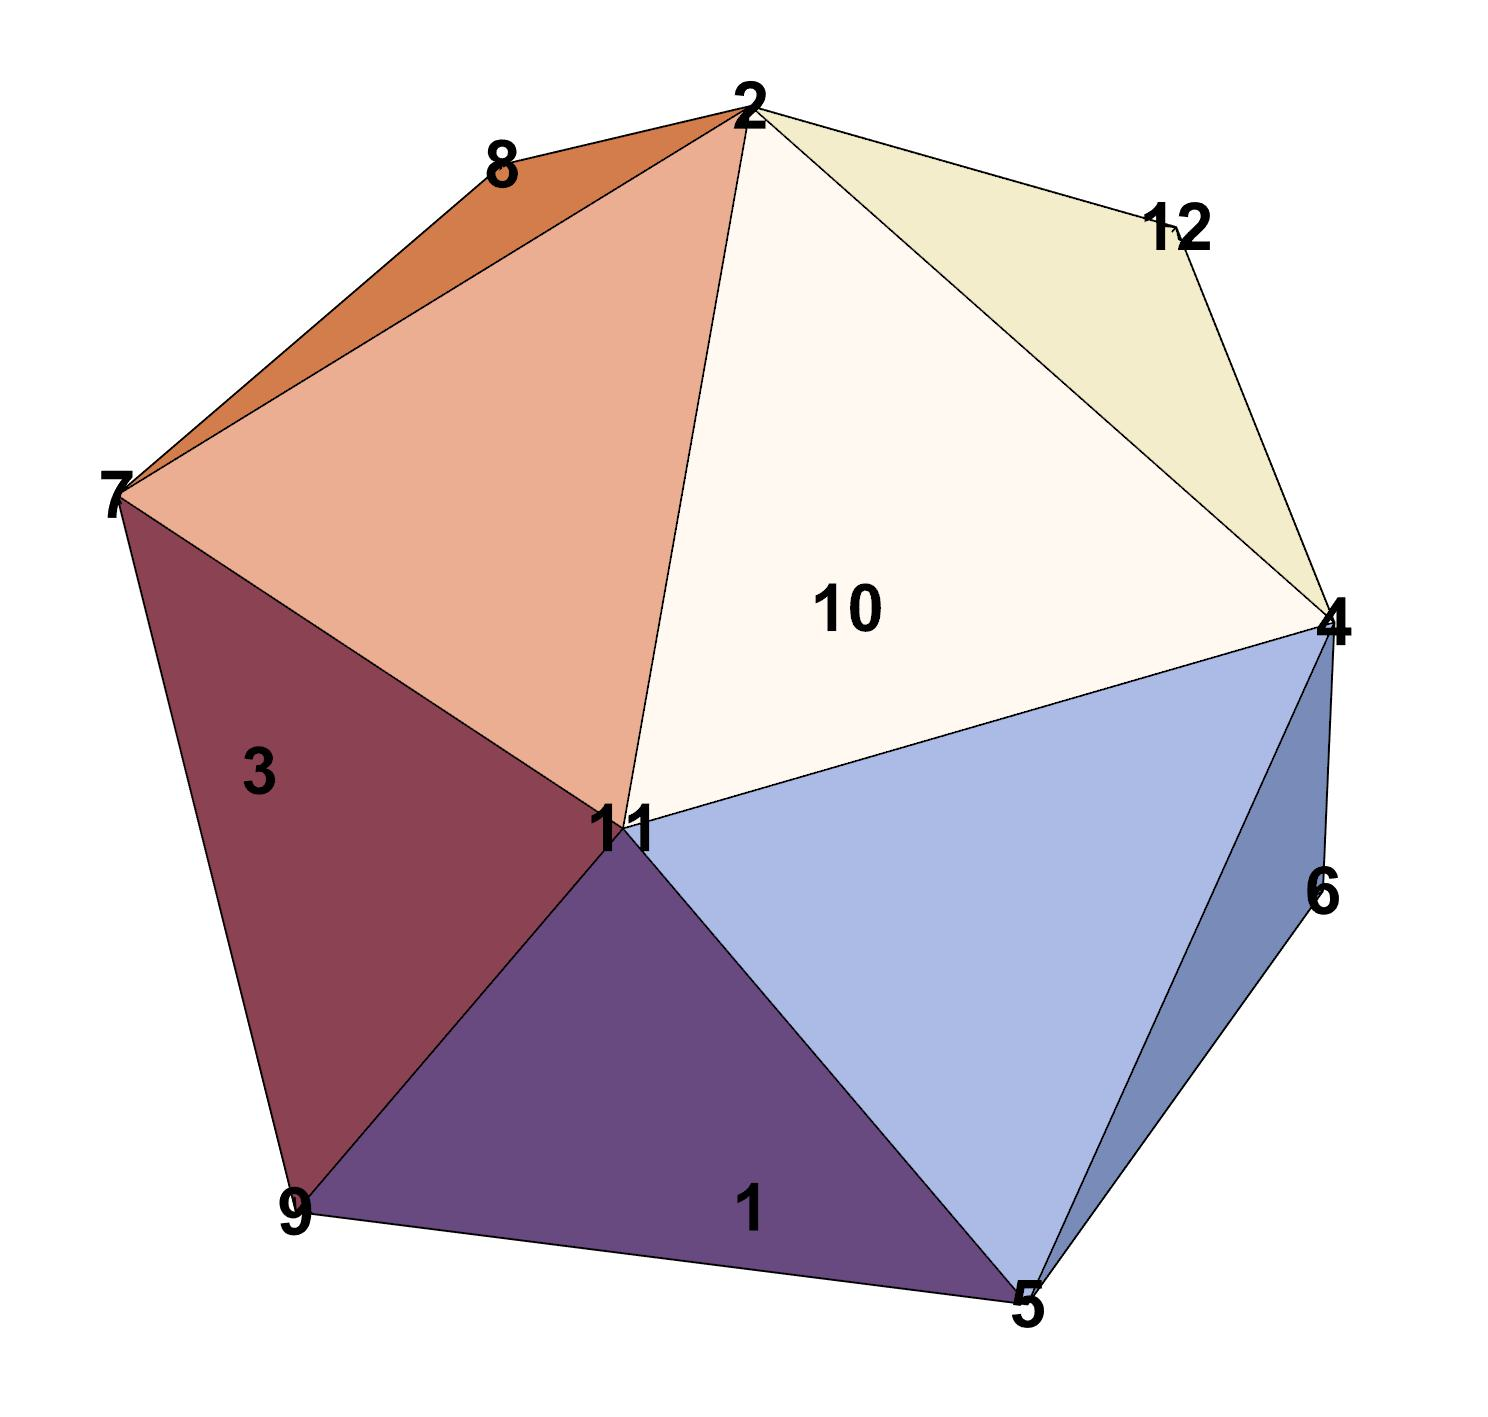
\includegraphics[width=0.45\textwidth]{icosahedron.jpg}
    \caption{Vertex labeling of the icosahedron used in the TFIM study. Each site interacts with its 5 neighbors via antiferromagnetic Ising couplings.}
    \label{fig:icosahedron}
\end{figure}

As shown in the recent work by Parez and Witczak-Krempa~\cite{parez2024}, the forward reduction hypothesis (FRH) is always satisfied for reduced density matrices (RDMs) of two spins. Consequently, FRH alone cannot explain the emergence of many-body scars on this lattice. However, for four- and five-spin RDMs (but not for three-spin RDM!), the FRH condition is no longer satisfied for certain eigenstates. The four and five spins are chosen to correspond to vertices on respectively two and three adjacent plaquettes of the icosahedron. In particular, five nearly degenerate scarred eigenstates appear at negative integer energy $E = -6$ for the antiferromagnetic model, and at integer energy $E = +6$ for the ferromagnetic one, with indices $[1267,1268,1269,1270,1271]$ and $[2826,2827,2828,2829, 2830]$ respectively. By changing the magnitude of TFIM parameters $J,h$ the position and properties of the scarred states do not change; the only thing that seems to affect the position of these scars is the sign of the coupling constant $J$, since that the energy of these scars changes sign between the ferromagnetic and antiferromagnetic model. All of these considerations suggest that the presence of these scars, as well their 5-fold degeneracy, is a direct consequence of the symmetry properties of the icosahedron (\textcolor{red}{create a perturbed version of the code with XY perturbation - ie not Ising - but with icosahedral symmetry, for both ferro and antiferro tfim. if this is true scars should persist}).

\begin{figure}[h]
    \centering
    \begin{minipage}{0.45\textwidth}
        \centering
        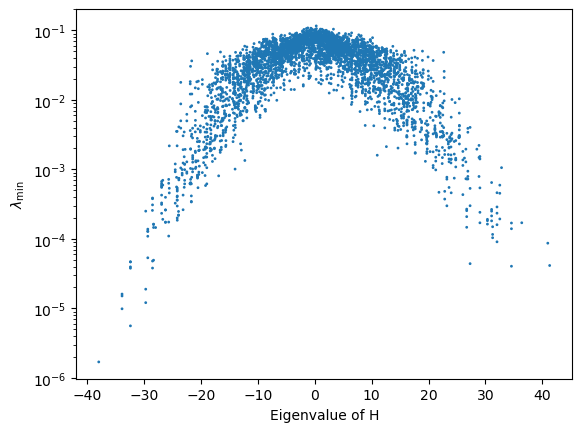
\includegraphics[width=\linewidth]{3spins.png}
    \end{minipage}\hfill
    \begin{minipage}{0.45\textwidth}
        \centering
        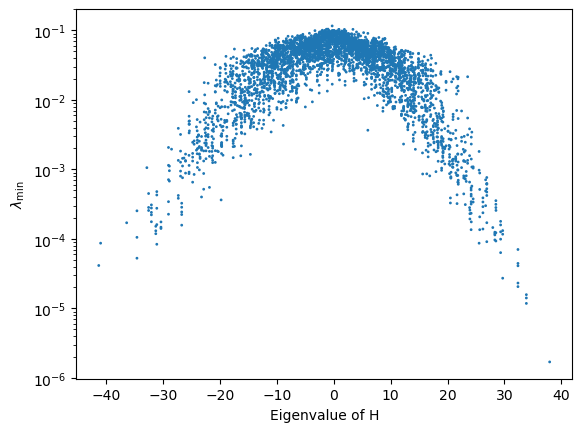
\includegraphics[width=\linewidth]{3spins-ferro.png}
    \end{minipage}
    \caption{Minimum eigenvalue of the three-spin RDM as a function of the eigenvalue of the Hamiltonian $H$, for the antiferromagnetic (left) and ferromagnetic (right) TFIM. In both cases, FRH is always satisfied; all eigenvalues remain well above machine precision.}
    \label{fig:3spins}
\end{figure}

\begin{figure}[h]
    \centering
    \begin{minipage}{0.45\textwidth}
        \centering
        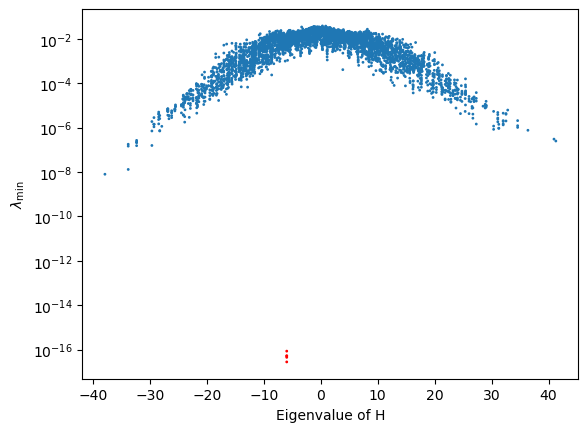
\includegraphics[width=\linewidth]{4spins.png}
        \caption{Minimum eigenvalue of the four-spin RDM for the antiferromagnetic TFIM. Five eigenstates (in red) near $E = -6$ violate FRH with eigenvalues $\lambda_{\min} \sim 10^{-16}$. These correspond to scarred states.}
        \label{fig:4spins_anti}
    \end{minipage}\hfill
    \begin{minipage}{0.45\textwidth}
        \centering
        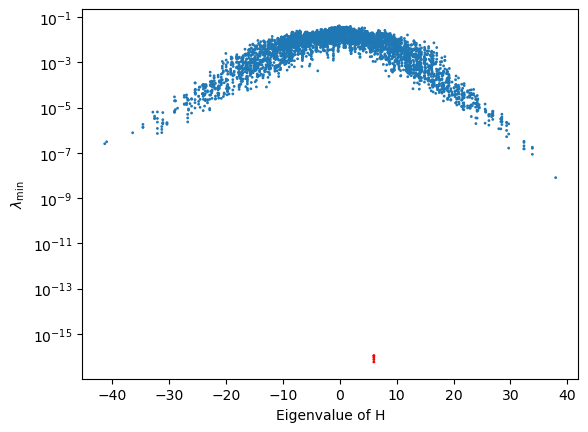
\includegraphics[width=\linewidth]{4spins-ferro.png}
        \caption{Minimum eigenvalue of the four-spin RDM for the ferromagnetic TFIM. Now the five scarred eigenstates have shifted to $E = +6$, suggesting a possible dependence on the sign of $J$.}
        \label{fig:4spins_ferro}
    \end{minipage}
\end{figure}


\begin{figure}[h]
    \centering
    \begin{minipage}{0.45\textwidth}
        \centering
        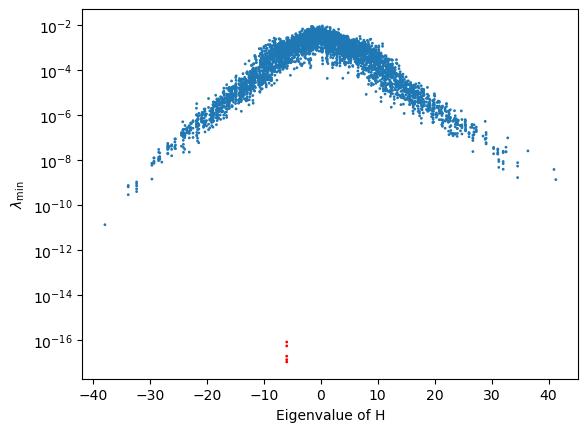
\includegraphics[width=\linewidth]{5spins.png}
        \caption{Minimum eigenvalue of the five-spin RDM for the antiferromagnetic TFIM. The five scarred eigenstates (in red) are still present at $E = -6$.}
        \label{fig:5spins_anti}
    \end{minipage}\hfill
    \begin{minipage}{0.45\textwidth}
        \centering
        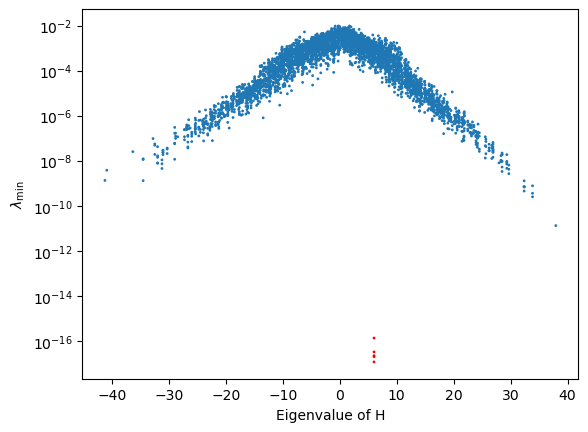
\includegraphics[width=\linewidth]{5spins-ferro.png}
        \caption{Minimum eigenvalue of the five-spin RDM for the ferromagnetic TFIM. The five scarred eigenstates are still present at $E = +6$.}
        \label{fig:5spins_ferro}
    \end{minipage}
\end{figure}

Let us analyze the properties of these scars, by looking at their entanglement properties (via bipartite entanglement entropy), the rank of their respective RDMs, and how they transform under the icosahedral point group  symmetry transformations $I_h$ (specifically, having five degenerate scars suggest to look at $C_5$).\\

\subsection{Entanglement entropy}

The bipartite entanglement entropy is computed for the whole spectrum, for the antiferromagnetic and ferromagnetic TFIM, and we look at the specific values of the scarred states. In both cases, only one of the five scars has an EE value that is smaller than that of the states in the bulk of the spectrum, specifically the scar with index 1268 for the antiferromagnetic model, with $EE \simeq 3.08$ and the scar with index 2827 for the ferromagnetic model, with $EE \simeq 3.36$. Given that the scars are degenerate, we can also take a linear combination (with complex coefficients) of all of them and compute the entanglement entropy of this new state. Numerically, we found that by optimizing the coefficients, the minimal value of EE obtained corresponds to $EE \simeq 1\times10^{-6}$ fo the antiferromagnetic TFIM and $EE \simeq 9\times10^{-7}$ for the ferromagnetic TFIM. Therefore, these optimal linear combinations seem to be badly scarred, much more of the single scars.

\begin{figure}[h]
    \centering
    \begin{minipage}{0.45\textwidth}
        \centering
        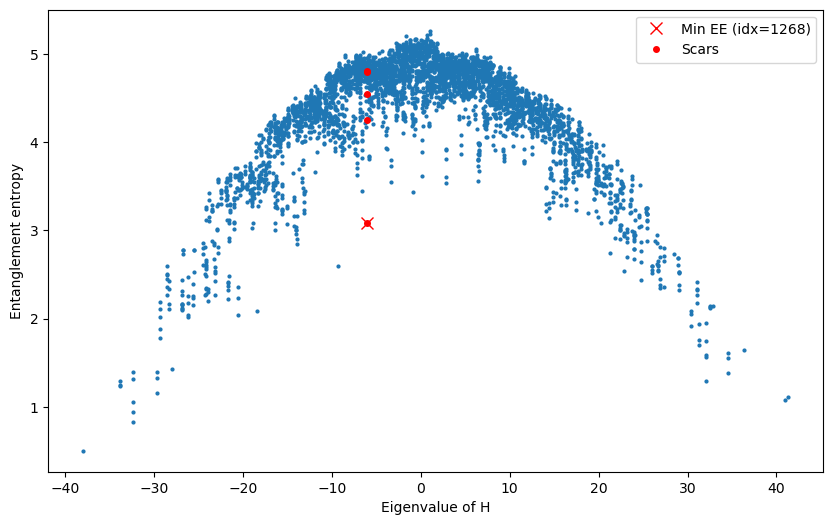
\includegraphics[width=\linewidth]{ee_anti.png}
        \caption{Bipartite entanglement entropy for the whole spectrum of the antiferromagnetic TFIM. The five scarred eigenstates (in red) have EE values similar to those of the states in the bulk, except for one state.}
        \label{fig:ee_anti}
    \end{minipage}\hfill
    \begin{minipage}{0.45\textwidth}
        \centering
        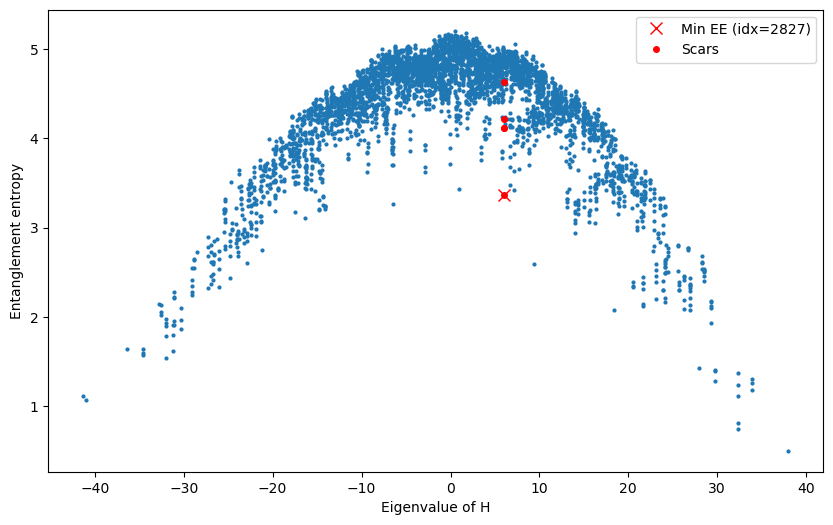
\includegraphics[width=\linewidth]{ee_ferro.png}
        \caption{Bipartite entanglement entropy for the whole spectrum of the ferromagnetic TFIM. Again, the five scarred eigenstates (in red) have EE values similar to those of the states in the bulk, except for one state.}
        \label{fig:ee_ferro}
    \end{minipage}
\end{figure}

\subsection{RDMs rank}

The four- and five-spins RDMs of the five scars have at least a vanishing eigenvalue, so their rank is not going to be full. Let us compute the rank in both cases, and understand why it is not full.

\begin{itemize}

\item \textbf{4 spins}: all of the five scars have 4-spins RDM rank equal to $\mathbf{11}$. The full rank of a 4-spins RDM is 16, so there are \textbf{five} columns of the RDM that are either zero or linearly dependent. Upon inspection of the null space of the matrix, we found that it actually corresponds to the five-dimensional totally symmetric subspace of $S_4$, the permutation group of 4 elements. In our case, the elements are $1/2$ spins, and the totally symmetric subspace correspond to states with total spin $S=2$. In other words, the 4-spins RDM doesn't have support on this subspace, suggesting that the global, 12-spins state must have some antisymmetry properties under the 12-spins permutation group $S_{12}$ instead.

\item \textbf{5 spins}: all of the five scars have 5-spins RDM rank equal to $\mathbf{18}$. The full rank of a 5-spins RDM is 32, so there are \textbf{fourteen} columns of the RDM that are either zero or linearly dependent. The totally symmetric subspace of 5 $1/2$ spins has dimension 6, so there are still 8 dimensions not accounted for. \textcolor{red}{explain}

\end{itemize}

The study of rank of 4- and 5-spins RDMs gave us valuable information regarding the global properties of the scarred states, hinting at a possible antisymmetric structure of such states under the 12-spins permutation group $S_{12}$. In fact, after a careful analysis of the numerical structure of such states, we were able to show that all scarred states (and only them) have exactly 6 spins up and 6 spins down, and 280 non-zero components. Looking at the non-zero components, they seem to appear in 140 pairs, with each pair made up of a positive coefficient and its negative version.\\
All of this suggests that the scarred states belong to the pair-wise antisymmetric subspace of $S_{12}$, which is denoted by $[6,6]$ using Young tableaux notation.\\
Note that RDMs rank considerations are applicable to both the antiferromagnetic and ferromagnetic TFIM model, with the only difference being that in the ferromagnetic model the alternating signs of the global scarred states are inverted and the magnitude of the coefficients changes, but the global states still belong to the [6,6] subspace.
The reason why the 5 scarred states belong to $[6,6]$ needs yet to be explained, but it's most likely due to the interaction of the permutation group $S_{12}$ and the icosahedron symmetry group $I_h$. 
 
\subsection{$C_5$ transformation properties}

The scarred states not only have special properties under the global permutation group $S_{12}$, but also under the cyclic group $C_5$ (five-fold rotations of the icosahedron about an axis passing through opposite vertices). In fact, the 5 scarred states belong to distinct 1-dimensional irreducible representations of $C_5$, or in other words, they are eigenvectors of $C_5$ with distinct eigenvalues or phase factors. By writing the action of $C_5$ in the 12 spins basis as a $2^{12}\times2^{12}$ matrix, and diagonalizing it in the degenerate scarred subspace, we found that:

\begin{equation}
\tilde{C}_5 |m\rangle = \exp^{i \frac{2\pi}{5} m} |m\rangle \quad m = 0,1,2,3,4
\end{equation} 

where $\tilde{C}_5$ is the $2^{12}\times2^{12}$ matrix representation of $C_5$, and we already know that the scarred eigenstates of the TFIM Hamiltonian are also eigenstates of $C_5$ because the Hamiltonian is symmetric under $C_5$ ($[H,C_5]=0$). We found that he antiferromagnetic and the ferromagnetic TFIM scars have the following values of $m$:

\begin{itemize}

\item antiferromagnetic TFIM: $[1267,1268,1269,1270,1271] \equiv [m=2,m=3,m=1,m=4,m=0]$

\item ferromagnetic TFIM: $[2826,2827,2828,2829, 2830] \equiv [m=0,m=1,m=4,m=2,m=3]$

\end{itemize}


The TFIM model on the icosahedron is not scalable, and therefore not relevant in the thermodynamic limit. It is however a toy model to understand how scars arise from symmetries, and it provides a useful introduction for more complicated models with many body quantum scars, such as the following.

\section{AKLT Model}

use hamiltonian with notation of the paper and outline the properties of the tower of exact scarred states - the aim of this section is to understand why these states have very low rank (inspection of null space for example). note that it's just not the tower states that don't have full rank, but some other states have almost full rank, but not full rank.

\section*{Bibliography}
\begin{thebibliography}{9}
    \bibitem{sachdev2011} S. Sachdev, \textit{Quantum Phase Transitions}, Cambridge University Press (2011).
    \bibitem{turner2018} C. J. Turner, A. A. Michailidis, D. A. Abanin, M. Serbyn, and Z. Papic, ``Quantum many-body scars," Nature Physics 14, 745–749 (2018).
    \bibitem{lieb1961} E. H. Lieb, T. Schultz, and D. Mattis, ``Two soluble models of an antiferromagnetic chain," Annals of Physics 16, 407-466 (1961).
    \bibitem{parez2024} G. Parez, W. Witczak-Krempa, ``The Fate of Entanglement," arXiv preprint arXiv:2402.06677 (2024).
\end{thebibliography}

\end{document}
